\begin{frame}{Fit in a non-SM scenario}
    \begin{columns}[b, onlytextwidth]
    \begin{column}{0.6\textwidth}
        \begin{tikzpicture}[remember picture,overlay]
            \node[anchor=west,inner sep=0pt] at ($(current page.west) + (0.15, 0)$) {
                \only<1>{
                    \begin{tabular}{rl}
                    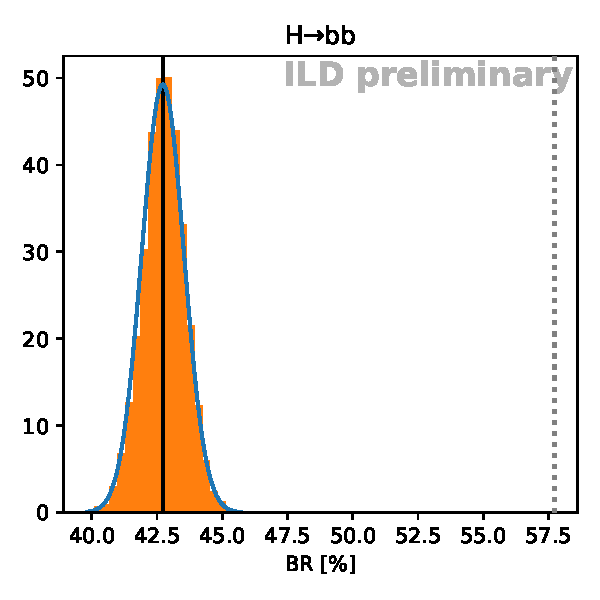
\includegraphics[width=0.45\textwidth]
                        {changed_toy_H_bb} &
                    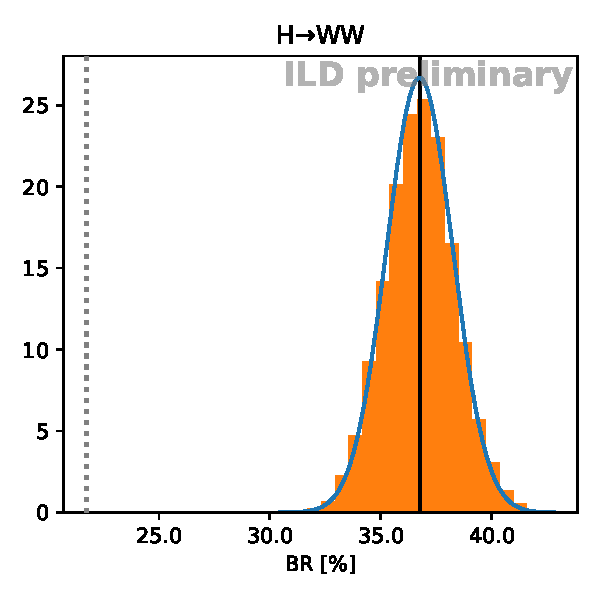
\includegraphics[width=0.45\textwidth]
                        {changed_toy_H_WW}
                    \end{tabular}
                }};
            \node[anchor=west,inner sep=0pt] at ($(current page.west) + (0.5, 0)$) {
                \only<2>{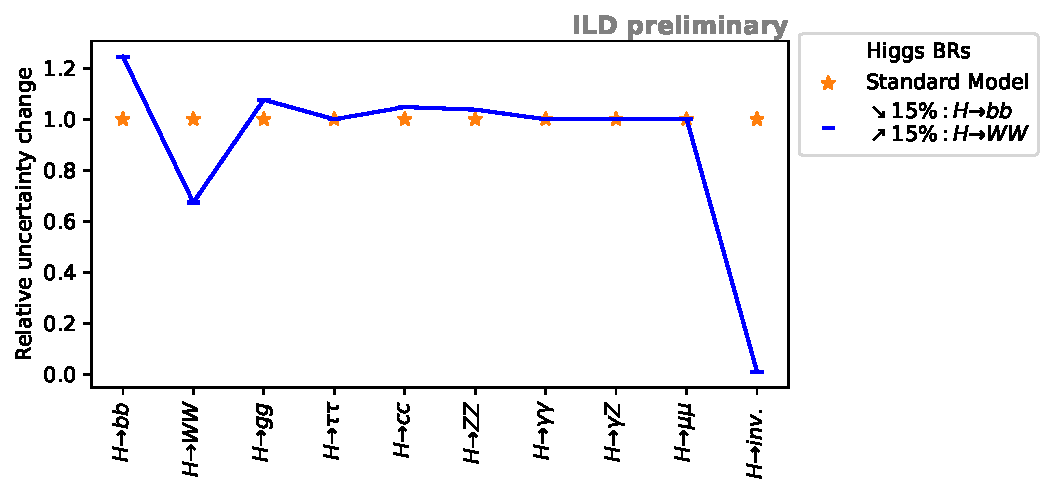
\includegraphics[width=\textwidth, keepaspectratio]
                {comparison_br_scenarios_1}}};
            \node[anchor=west,inner sep=0pt] at ($(current page.west) + (0.5, 0)$) {
                \only<3>{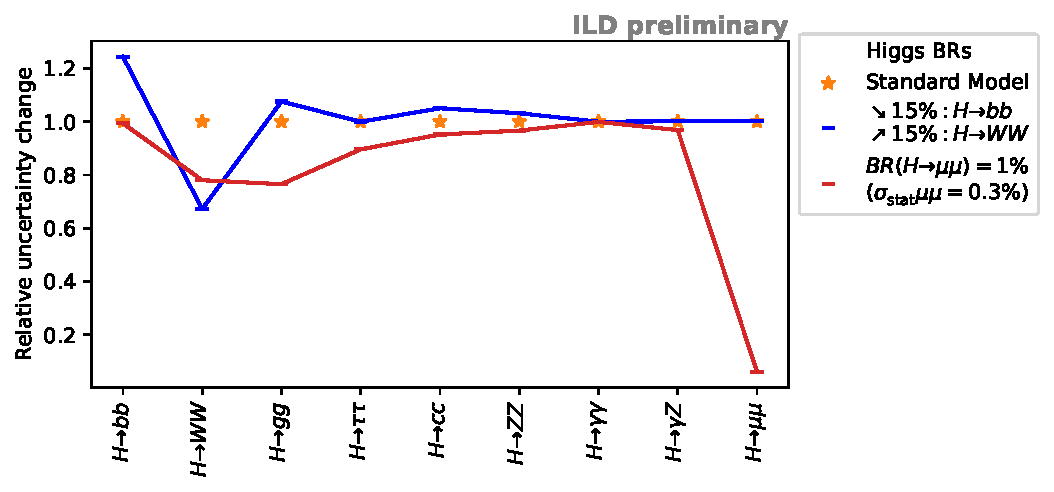
\includegraphics[width=\textwidth, keepaspectratio]
                {comparison_br_scenarios_2}}};
    \end{tikzpicture}
        Assume $57.7\% \to 42.7\%$ $BR(H\to b\bar{b})$, \\
        \hspace{4em}$21.8\% \to 36.8\%$ $BR(H\to W^+W^-)$.
    \end{column}
    \begin{column}{0.38\textwidth}
    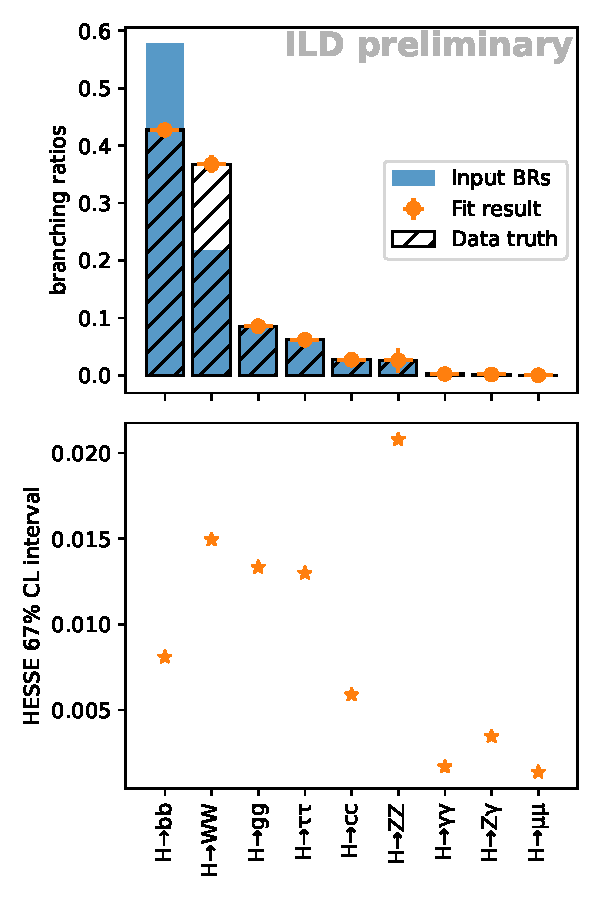
\includegraphics[height=0.85\textheight, keepaspectratio]
        {changed_br_estimates}
    \end{column}
    \end{columns}
    \end{frame}
